\documentclass[10pt]{article}
%\usepackage[utf8]{inputenc}
\oddsidemargin=0cm
\textwidth=15cm
\usepackage{graphicx}
%\usepackage[utf8x]{inputenc}
%\usepackage[spanish]{babel}
%\DeclareGraphicsExtensions{.bmp,.jpg}
\usepackage[latin1]{inputenc}
\usepackage{amsmath}
\usepackage{amsthm}
\usepackage{amsfonts}
\usepackage{adjustbox}
\usepackage{amssymb}
\usepackage[dvips]{epsfig}
\usepackage{ulem}
\usepackage{indentfirst}
\usepackage{wasysym}
\usepackage{pifont}
\usepackage{fancyhdr}
%\usepackage{color}
\usepackage{multicol}
\usepackage{framed}
\usepackage[usenames, dvipsnames]{color}
\usepackage{wrapfig}

%\textwidth=17cm %ancho del texto, de paso define margen de la derecha
%\topmargin=2cm %margen superior
%\oddsidemargin=-0.5cm %margen de la izquierda del texto
%\evensidemargin=0.5cm 

%\definecolor{color1}{RGB}{220,250,250}
\definecolor{shadecolor}{RGB}{220,250,250}
%238
\pagestyle{myheadings}
\definecolor{color1}{RGB}{220,250,250}
\definecolor{color2}{rgb}{0.99,0.9,1.0}
\definecolor{color3}{RGB}{220,250,250}
\definecolor{color4}{rgb}{0.0,0.5,0.69}
\definecolor{color5}{rgb}{1.0,1.0,0.88}
\definecolor{color6}{rgb}{1.0,0.94,0.84}
\definecolor{color7}{rgb}{0.94,1.0,1.0}
\definecolor{color8}{rgb}{1.0,0.94,0.84}
\definecolor{color9}{rgb}{0.0,0.5,0.69}
\definecolor{dblue}{rgb}{1.0,0.0,1.0}
\definecolor{dred}{rgb}{1.0,0.0,0.0}
\definecolor{lred}{rgb}{0.82,0.1,0.26}

%HIGHLIGHT 2 (turquise)
\newcommand{\2}[1]{\hspace{-0.93cm}\colorbox{color1}{\hspace{0.07cm} \parbox{17cm}{\vspace{0.2cm} #1}\hspace*{0.07cm} }}

%HIGHLIGHT 3 ()
\newcommand{\3}[1]{\hspace{-0.93cm}\colorbox{color7}{\hspace{0.07cm} \parbox{17cm}{\vspace{0.2cm} #1}\hspace*{0.07cm} }}
%NOTA
\newcommand{\nota}[1]{\textbf{Notaci\'on:}\: 
#1}

%LINE
\newcommand{\start}{\noindent {\color{color4}\rule{17cm}{0.5mm}}\\}

%Notation
\newcommand{\notation}[1]{\begin{framed}\noindent \nota{#1} \end{framed}}

%COMIENZO
\newcommand{\com}[1]{\noindent\rule{17cm}{0.8mm}
\begin{center}
\textbf{{\Large #1}}
\end{center}
\noindent\rule{17cm}{0.8mm}\\
}

%DEMOSTRACION
\newcommand{\dem}{\noindent {\color{color4}\rule{17cm}{0.5mm}}\\ \negrita{\textbf{Demostraci\'on: }}} 


%REFLEXION
\newcommand{\reflexion}[1]{\2{\textbf{\underline{Reflexi\'on.}}\\

#1\\}\\ }

%NEGRITA
\newcommand{\negrita}[1]{{\color{color4}\textbf{#1}}}

\newcommand{\red}[1]{{\color{red}\textbf{#1}}}

%HIGHLIGHT
\newcommand{\highlight}[1]{\begin{shaded} #1 \end{shaded}}

%FRAME
\newcommand{\enmarcar}[1]{\begin{framed} #1 \end{framed}}


%OBSERVATION 
\newcommand{\obs}[1]{\textbf{Observati\'on:} #1}

%HIGHLIGHT 2
\newcommand{\Highlight}[1]{\hspace{-0.93cm}\colorbox{color9}{\hspace{0.07cm} \parbox{12.7cm}{\vspace{0.2cm} #1}\hspace*{0.07cm} }}

% DESAFIO
\newcommand{\Desafio}[1]{\noindent\rule{13.3cm}{0.4mm}\\
\Highlight{ #1
\vspace{0.3cm} }
\noindent\rule{13.3cm}{0.3mm}\\}

%OBSERVATION
\newcommand{\observation}[1]{\begin{framed} \obs{#1} \end{framed}}

%SOLUTION
\newcommand{\sol}{\noindent {\color{color4}\rule{13.3cm}{0.5mm}}\\ \negrita{\textbf{Soluci\'on: }}} 

%\markboth{}{Construcci\'on de Tesis}

%\title{Control 1 de Matem\'aticas 1}
%\author{Programa de Bachillerato. Universidad de Chile.}
%\date{Lunes 24 de Marzo, 2013}
\theoremstyle{theorem}
\newtheorem{teo}{\textbf{Teorema}}%[chapter]
\newtheorem{lema}{\textbf{Lema}}%
\newtheorem{defi}{\textbf{Definici\'on}}%[chapter]
\newtheorem{propi}{Propiedad}%[chapter]
\newtheorem{propir}{Propiedad Relevante}%[chapter]
\newtheorem{pro}{Proposici\'on}%[chapter]
\newtheorem{ax}{Axioma}
\newtheorem{prob}{Problema}
\newtheorem{eje}{Ejemplo}%[chapter]
\newtheorem{ejer}{\textsc{Ejercicio}}%[section]
\newtheorem{ejerr}{Ejercicio Resuelto}
\newtheorem{obser}{Observaci\'on}%[chapter]
\newcommand{\R}{\mathbb{R}} 
\newcommand{\Z}{\mathbb{Z}}
\newcommand{\Q}{\mathbb{Q}}
\newcommand{\C}{\mathbb{C}}
\newcommand{\N}{\mathbb{N}}
\newcommand{\U}{\mathbb{U}}
\newcommand{\D}{\mathbb{D}}
\newcommand{\I}{\mathbb{I}}
\numberwithin{equation}{section}
\pagestyle{myheadings}
\usepackage{enumerate}
\newcommand{\dis}{\displaystyle}
\usepackage[all]{xy}
\usepackage{tabu}  %paquete para hacer tablas

\title{C\'alculo Diferencial (MAT170)\\ Clase 7 }
\author{Prof. Marco Godoy\\
marco.godoy@edu.udla.cl}
\date{Abril 2019}

\begin{document}


\maketitle

\section{Identidades trigonom\'etricas}

Las identidades trigonom\'etricas m\'as usadas, a la hora de resolver problemas son las siguientes:

\begin{enumerate}[1.]

\item Las usuales, asociadas al teorema de Pit\'agoras en el c\'irculo unitario:

\begin{align*}
  \sin^2(\alpha)+\cos(\alpha)&=1,\\
  1+\tan^2(\alpha)&=\sec^2(\alpha),\\
  1+\cot^2(\alpha)&=\csc^2(\alpha).
\end{align*}

\item Suma de \'angulos:

\begin{align*}
\sin(\alpha+\beta)&=\sin(\alpha)\cos(\beta)+\sin(\beta)\cos(\alpha),\\
\cos(\alpha+\beta)&=\cos(\alpha)\cos(\beta)-\sin(\alpha)\sin(\beta).
\end{align*}

\begin{eje}
Ocupando las identidades trigonom\'etricas de arriba, demuestre lo siguiente: $$\frac{\cos(\alpha)}{1+\sin(\alpha)}+\frac{1+\sin(\alpha)}{\cos(\alpha)}=2\sec(\alpha).$$

\end{eje}

\textbf{Desarrollo.} Este es un trabajo netamente algebraico:

\begin{align*}
\frac{\cos(\alpha)}{1+\sin(\alpha)}+\frac{1+\sin(\alpha)}{\cos(\alpha)}&=\frac{\cos^2(\alpha)+(1+\sin(\alpha))^2}{\cos(\alpha )(1+\sin(\alpha))}\\
&=\frac{\cos^2(\alpha)+1+\sin^2(\alpha)+2\sin(\alpha)}{\cos(\alpha )(1+\sin(\alpha))}\\
&=\frac{1+(\cos^2(\alpha)+\sin^2(\alpha))+2\sin(\alpha)}{\cos(\alpha )(1+\sin(\alpha))}\\
&=\frac{2+2\sin(\alpha)}{\cos(\alpha )(1+\sin(\alpha))}\\
&=\frac{2(1+\sin(\alpha))}{\cos(\alpha )(1+\sin(\alpha))}\\
&=\frac{2}{\cos(\alpha )}\\
&=2\sec(\alpha)
\end{align*}

Por lo tanto, se cumple que $\dis \frac{\cos(\alpha)}{1+\sin(\alpha)}+\frac{1+\sin(\alpha)}{\cos(\alpha)}=2\sec(\alpha).$

\end{enumerate}


\section{Gr\'afica de funciones trigonom\'etricas y ecuaciones trigonom\'etricas}

Una \textbf{ecuaci\'on trigonom\'etrica} es una ecuaci\'on en el que est\'a involucrada alguna funci\'on trigonom\'etrica. Por ejemplo:

\begin{align*}
\sin(x^2)+x^2&=1+x,\\
\cos(x+5)&=\sin(x)+6.
\end{align*} 

En el contexto de este curso, s\'olo nos interesa resolver ecuaciones trigom\'etricas del tipo:
\begin{align}\label{ecs}
\sin(\alpha)&=a,\\
\cos(\beta)&=b,\label{ecs2}
\end{align}
donde $\alpha,\beta\in [0,2\pi]$ y $a,b\in [-1,1]$. Por lo que \textbf{toda ecuaci\'on trigom\'etrica que aparezca en un problema debe ser transformada, mediante operaciones algebraicas e identidades trigonom\'etricas, a una ecuaci\'on trigonom\'etrica del tipo \ref{ecs} o \ref{ecs2}.}
Para saber c\'omo resolver c\'omo resolver las ecuaciones trigonom\'etricas \ref{ecs}, \ref{ecs2}, se necesita saber los gr\'aficos de las funciones seno y coseno en el intervalo $[0,2\pi]$

\begin{figure}[h!]
\centering
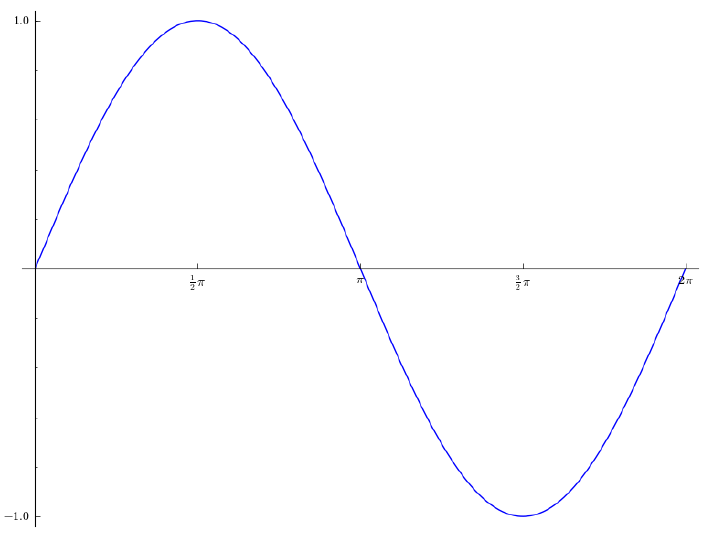
\includegraphics[scale=0.3]{sine}
\caption{Gr\'afica de la funci\'on seno en $[0,2\pi]$}
\label{sine}
\end{figure}

\begin{figure}[h!]
\centering
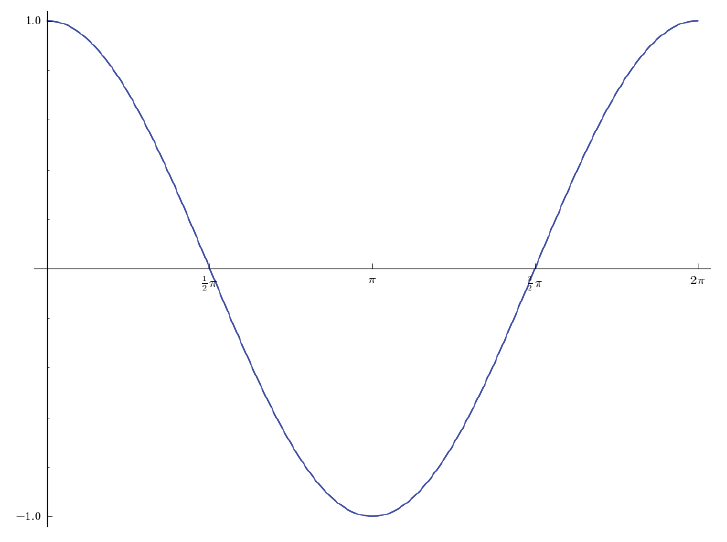
\includegraphics[scale=0.3]{cosine}
\caption{Gr\'afica de la funci\'on coseno en $[0,2\pi]$}
\label{cosine}
\end{figure}

\begin{pro}\label{soluciones ecua}
Se cumple:
\begin{enumerate}[1.]
   \item $\sin(\pi-\alpha)=sin(x)$,
   \item $\cos(2\pi - \alpha)=\cos(\alpha)$.
\end{enumerate}
\end{pro}
Con ayuda de la Proposici\'on \ref{soluciones ecua}, m\'as la ayuda de las Figuras \ref{sine},\ref{cosine}:

\begin{pro} Se cumple:
\begin{enumerate}[1.]
   \item Si $\alpha=\alpha_0$ es una soluci\'on de la ecuaci\'on $\sin(\alpha)=a$ para $\alpha \in [0,2\pi]$, es decir $$\sin(\alpha_0)=a,$$ entonces $\alpha=\pi-\alpha_0$ tambi\'en es una soluci\'on de la ecuaci\'on. El n\'umero $\alpha_0$ se escribe como $$\alpha_0=\arcsin(a).$$ Se lee \textbf{el arcoseno de $a$}.
   \item Si $\alpha=\alpha_0$ es una soluci\'on de la ecuaci\'on $\cos(\alpha)=b$ para $\alpha \in [0,2\pi]$, es decir $$\cos(\alpha_0)=b,$$ entonces $\alpha=2\pi-\alpha_0$ tambi\'en es una soluci\'on de la ecuaci\'on. El n\'umero $\alpha_0$ se escribe como $$\alpha_0=\arccos(b).$$ Se lee \textbf{el arcocoseno de $b$}.
\end{enumerate}
\end{pro}

\begin{eje}
Resuelva la siguiente ecuaci\'on trigonom\'etrica: $$\sin(2\alpha)-\sin(\alpha)=0,$$ en el intervalo $[0,2\pi]$.
\end{eje}

\section{Problemas propuestos}

\begin{enumerate}[P1.]
    \item Demuestre que $\dis \tan(\alpha+\beta)=\frac{\tan(\alpha)+\tan(\beta)}{1-\tan(\alpha)\tan(\beta)}$.
    \item Para el intervalo $[0,2\pi]$, resuelva las siguientes ecuaciones:
    \begin{enumerate}[1.]
       \item $\dis \cos(x)=\frac{2\tan(x)}{1+\tan^2(x)}$
       \item $\cos(2x)=\sin(x)$
       \item $\cos(2x)+\cos(-x)=0$.
    \end{enumerate}     
\end{enumerate}
\end{document}